\documentclass[12pt,a4paper]{article}
\usepackage[utf8]{inputenc}
\usepackage[russian]{babel}
\usepackage{amsmath}
\usepackage{amsfonts}
\usepackage{amssymb}
\usepackage{graphics}
\usepackage[pdftex]{graphicx}
\usepackage{lscape}
\usepackage{listings}
\usepackage{geometry} % Меняем поля страницы
\geometry{left=2cm}% левое поле
\geometry{right=1.5cm}% правое поле
\geometry{top=2cm}% верхнее поле
\geometry{bottom=15mm}% нижнее поле
\RequirePackage{float}
\renewcommand{\baselinestretch}{1.5}
\pagestyle{plain}
\begin{document}
\thispagestyle{empty}
\begin{center}
\large Санкт-Петербургский государственный политехнический университет\\
Институт информационных технологий и управления\\
Кафедра компьютерных систем и программных технологий\\
\vspace{65mm}
\Large Реферат клабораторной работе №1\\ По предмету "Проектирование ОС и компонентов" \\на тему:\\
\LARGE\textbf{Работа с инструментарием}
\end{center}

\vspace{40mm}
\begin{flushright}
\large Выполнила: студентка группы 53501/3\\ Тарасова А. А.\\ Преподаватель: Душутина Е. В.
\end{flushright}
\vspace{30mm}

\begin{center}
Санкт-Петербург\\ 2015
\end{center} % это титульный лист
\newpage
\tableofcontents
\newpage
\section{VirtualBox}
	\textbf{VirtualBox} – это мощное кросс-платформенное средство для программной виртуализации на платформах на базе х86. «Кросс-платформенность» означает, что VirtualBox может быть установлен на компьютеры с MS Windows, Linux, Mac OS X и Solaris x86, а «средство для программной виртуализации» означает, что Вы можете создавать и запускать различные виртуальные машины, использующие различные операционные системы одновременно на одном компьютере. Например, Вы можете запустить Windows и Linux на Mac, или Linux и Solaris из-под Windows, или Windows из-под Linux.

Oracle VM VirtualBox доступна для загрузки в виде открытого кода или в виде установочных бинарных файлов для Windows, Linux, Mac OS X и Solaris.

Дистирибутив VirtualBox можно скачать по ссылке https://www.virtualbox.org/wiki/Downloads
\subsection{Создание виртуальной машины}
Внегний вид VirtualBox представлен на рисунке 1.
\begin{figure}[h!]
\centering
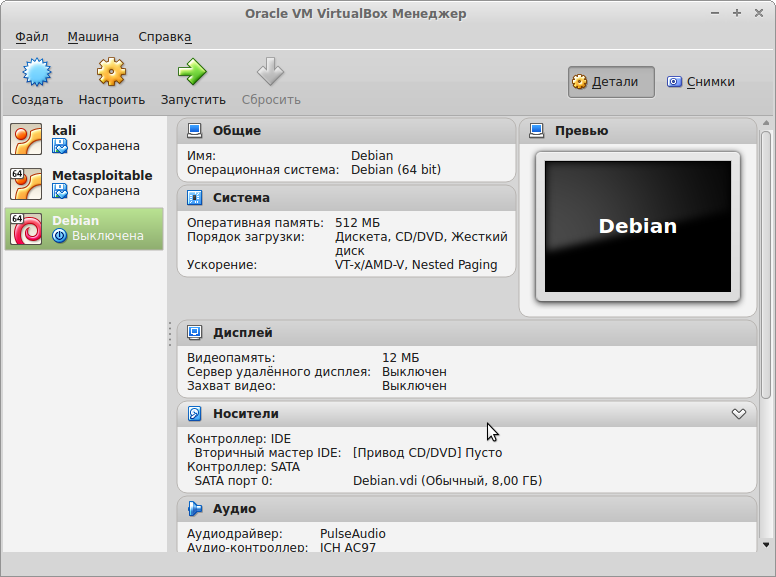
\includegraphics[scale=0.5]{res/VirtualBox}
\caption{VirtualBox}
\end{figure}

Для того чтобы создать виртуальную машину необходимо нажать кнопку \verb+Создать+. В окне, изображенном на рисунке 2 пишем название системы и выбираем её тип. В моём случае имя машины \verb+Debian+, тип \verb+Linux+, версия \verb+Debian (64bit)+.
\begin{figure}[h!]
\centering
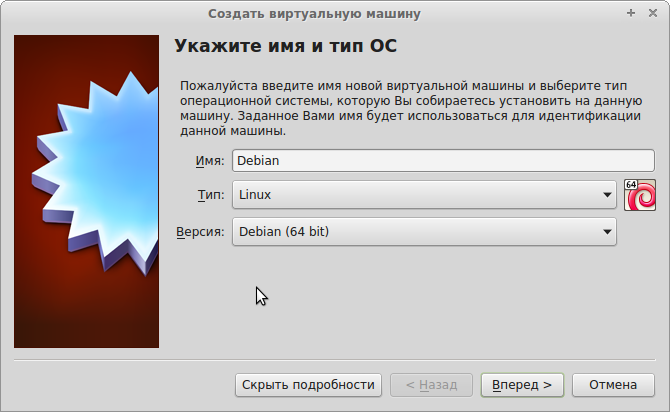
\includegraphics[scale=0.5]{res/CreateMaschine}
\caption{Создание виртуальной машины, выбор типа и версии}
\end{figure}

Затем, необходимо указать объем оперативной памяти (RAM), которая будет выделена данной виртуальной машине (рисунок 3).
\begin{figure}[h!]
\centering
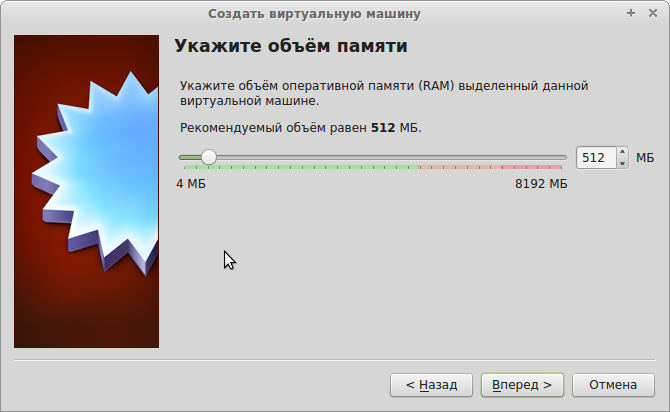
\includegraphics[scale=0.5]{res/RAMSize}
\caption{Выбор размера оперативной памяти}
\end{figure}

После этого необходимо определиться с жестким диском для виртуальной машины. В моем случае требуется \verb+Создать новый виртуальный жесткий диск+. Это показано на рисунке 4.
\begin{figure}[h!]
\centering
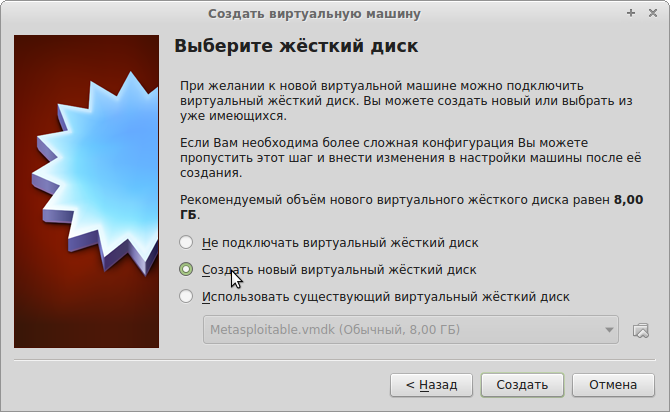
\includegraphics[scale=0.5]{res/ROM}
\caption{Выбор жесткого диска}
\end{figure}

Следующим этапом является выбор типа жесткого диска виртуальной машины.
Файлы дисковых образов располагаются на хост системе и определяются гостевыми системами как жесткие диски определенного размера. При чтении или записи данных с диска гостевой ОС, VirtualBox перенаправляет дисковые запросы к файлу образа.

Как и у физического диска, у виртуального диска есть размер, который надо указать при создании. В отличии от физических дисков, VirtualBox позволяет увеличивать образ файла после его создания.\\
VirtualBox поддерживает 4 типа файлов образов диска:
\begin{itemize}
\item Virtual Disk Image (VDI)-файлы - собственный формат виртуальных дисков.
\item VMDK - формат, использующийся в множестве других продуктах виртуализации (VMware).
\item VirtualBox таже полностью поддерживает формат VHD разработанный Microsoft.
\item Файлы образов Parallels 2 версии (HDD format) также поддерживаются. Новые версии этого формата (3 and 4) не поддерживаются.
\end{itemize}

По умолчанию будет использоваться нативный для VirtualBox формат — \verb+VDI+.

\begin{figure}[h!]
\centering
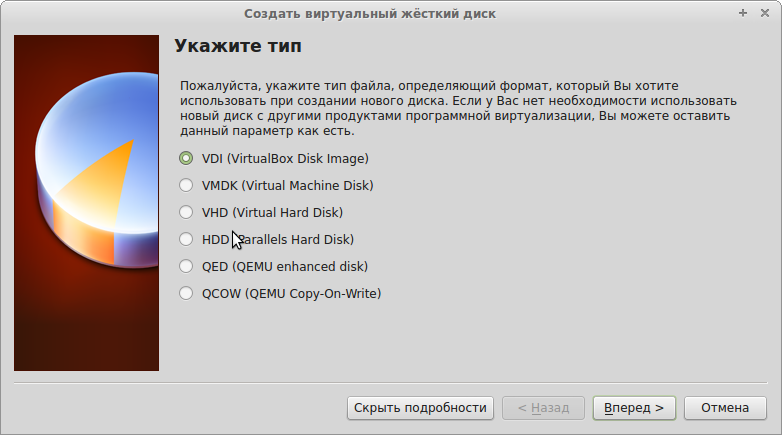
\includegraphics[scale=0.45]{res/TypeOfHardDrive}
\caption{Выбор типа жесткого диска}
\end{figure}

Следующим шагом будет выбор между динамическим и фиксированным типом диска.

Независимо от формата виртуальных дисков, существует два типа создаваемых образов: фиксированного размера и динамически расширяемые.
\begin{itemize}
\item Если вы создаете образ фиксированного размера емкостью 10 GB, то на хост системе будет создан файл примерно такого же размера. Создание фиксированных образов может занять довольно значительное время, в зависимости от размера образа и производительности дисковых операций системы.
\item Для более гибкого управления виртуальными носителями, используются динамически расширяемые образы . При создании данный образ будет иметь небольшой размер, за счет неиспользуемого пространства виртуального диска, но по мере использования, файл образа будет увеличиваться. Данный вид файла занимает меньше места на начальном этапе, однако VirtualBox необходимо увеличивать размер образа (пока образ не достигнет максимального размера), что ведет к замедлению дисковых операций по сравнению с дисками фиксированного размера. Однако, после достижения предела расширения динамического диска, потери производительности операций чтения и записи уже не так значительны.
\end{itemize}

В моем случае выбран \verb+динамический виртуальный жесткий диск+
\begin{figure}[h!]
\centering
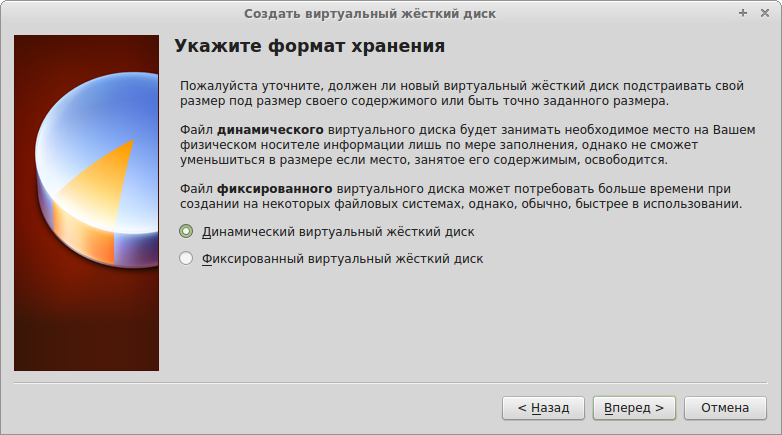
\includegraphics[scale=0.45]{res/StorageFormat}
\caption{Выбор формата хранения}
\end{figure}

После нажатия кнопки \verb+Создать+  будет создан виртуальный диск с выбранными параметрами.

\begin{figure}[h!]
\centering
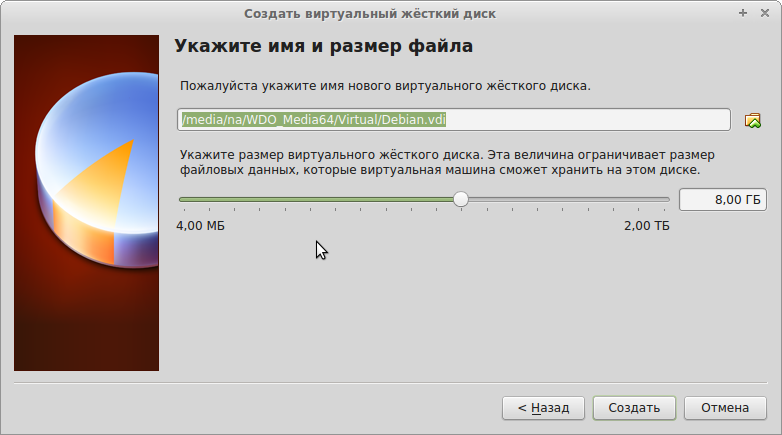
\includegraphics[scale=0.45]{res/WhereToInstall}
\caption{Выбор имя и размер файла виртуальной машины}
\end{figure}
\newpage
\subsection{Установка операционной системы на виртуальный диск}
Для начала следует зайти в \verb+Свойства+ и выбрать раздел \verb+Настроить+ (рисунок 8).
\begin{figure}[h!]
\centering
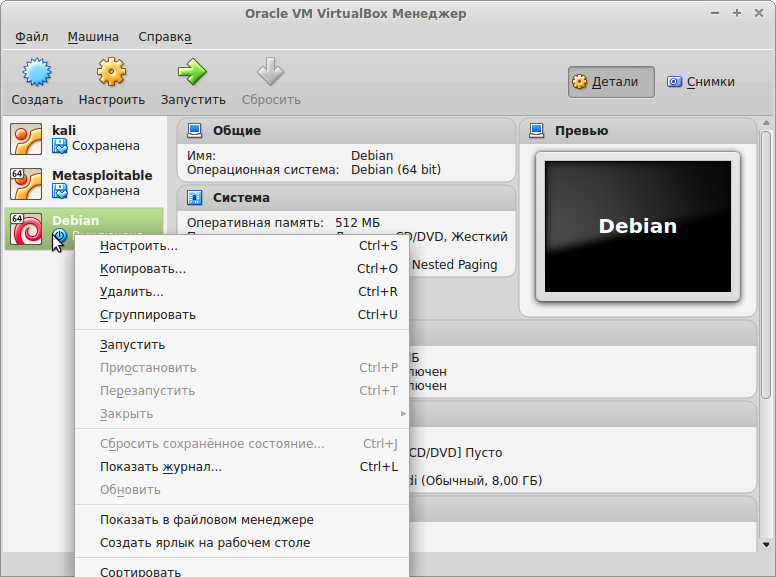
\includegraphics[scale=0.45]{res/Properties}
\caption{Заходим в настройки виртуальной машины}
\end{figure}

\begin{figure}[h!]
\centering
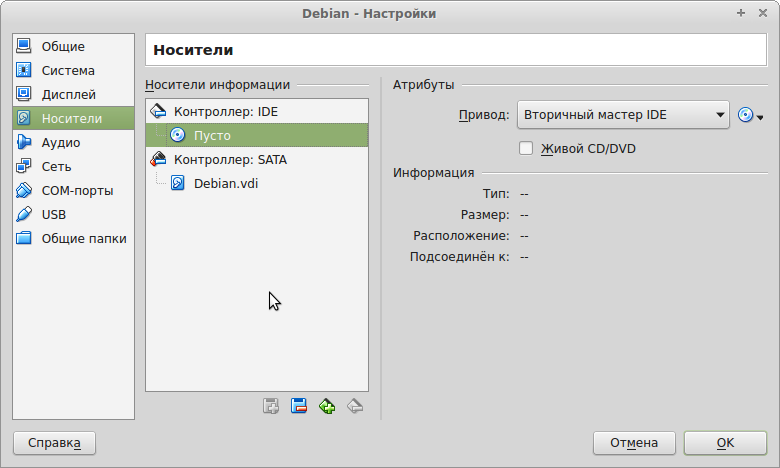
\includegraphics[scale=0.45]{res/carriers}
\caption{Заходим в настройки виртуальной машины}
\end{figure}

В блоке \verb+Контроллер ОС+ следует выбрать \verb+Пусто+, а в блоке \verb+Атрибуты+  нужно нажать на иконку CD диска. Появится список с требуемыми действиями. Если инсталляционный диск записан на CD/DVD диске, то надо выбрать пункт \verb+Привод хоста ‘Х:‘+, где Х это буква диска. В случае если ОС хранится в ISO-образе, то надо выбрать пункт  \verb+Выбрать образ оптического диска+ и указать на файл образа(рисунки 9, 10, 11).


\begin{figure}[h!]
\centering
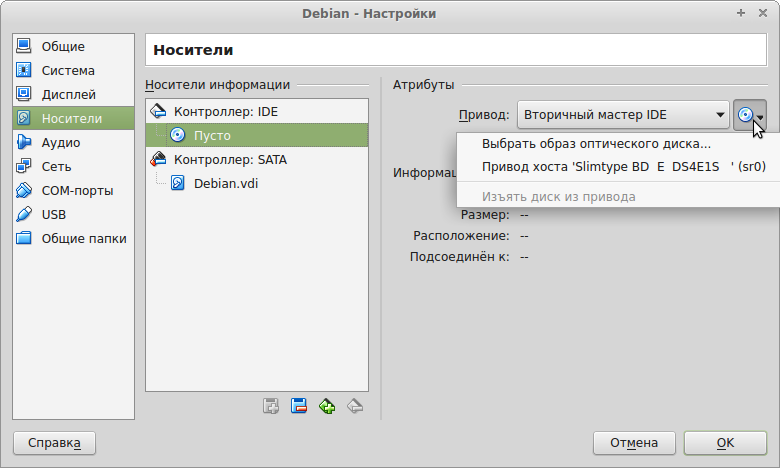
\includegraphics[scale=0.45]{res/choose}
\caption{Заходим в настройки виртуальной машины}
\end{figure}

\begin{figure}[h!]
\centering
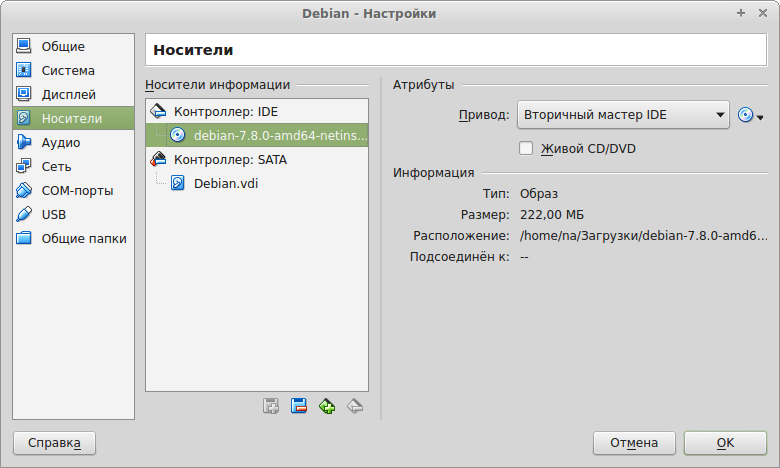
\includegraphics[scale=0.45]{res/chooseiso}
\caption{Заходим в настройки виртуальной машины}
\end{figure}

На этом настройка завершена. Никаких других настроек, в большинстве случаев, производить не надо. И сейчас уже можно запустить нашу виртуальную машину нажав на иконку «Старт». После процесса установки получим операционную систему работающую в виртуальной машине.

\newpage
\section{Архивы Debian}
Дистрибутив Debian можно скачать по ссылке https://www.debian.org/distrib/netinst
\subsection{Структура каталогов}
Следующие каталоги могут быть найдены на каждом зеркале Debian в каталоге debian:
\begin{itemize}
  \item dists/:

 Этот каталог содержит "дистрибутивы" и используется для канонического пути для доступа к имеющимся (в настоящее время) пакетам в релизах и пре-релизах Debian. Некоторые старые пакеты и файлы Packages.gz могут быть до сих пор и здесь.
  
  \item pool/:
  
  Это новое физическое расположение всех пакетов релизов и пре-релизов Debian.
  \item tools/:
  
  DOS-утилиты для создания загрузочных дискет, разбиения вашего жесткого диска, сжатия/распаковки файлов и загрузки Linux.
  \item doc/:
  
  Это основная документация по Debian, такая как FAQ, инструкции по системе оповещения об ошибках и т.д.
  \item indices/:
  
  The Maintainers file and the override files.
  
  \item project/: материалы, в основном, для разработчиков. Это:
      \begin{itemize}
        \item project/experimental/:
        
        Этот каталог содержит пакеты и инструменты, которые находятся в разработке или даже в альфа-тестировании. Пользователи не должны использовать эти пакеты, так как они могут быть опасны и вредны даже для достаточно опытных.
        \item project/orphaned/:
        
        Здесь находятся пакеты, которые 'осиротели' (т.е. остались без мейнтейнера) и были изъяты из дистрибутива.
      \end{itemize}
\end{itemize}
\subsection{Дистрибутивы Debian}
Обычно существует три дистрибутива Debian в каталоге dists. Это дистрибутив stable, дистрибутив testing и дистрибутив unstable. Иногда может быть еще и frozen. Каждый дистрибутив определяется как символическая ссылка на реальный каталог под кодовым именем в каталоге dists. 
\subsubsection{Дистрибутив stable}
Пакеты stable дистрибутива Debian записываются в каталог stable:
\begin{itemize}
  \item stable/main/: 
  
   Этот каталог содержит пакеты, которые формально составляют самый свежий релиз системы Debian.
  \item stable/non-free/:
  
  Этот каталог содержит пакеты, распространение которых ограничено требованиями ряда копирайтов.
  \item stable/contrib/:
  
  Этот каталог содержит пакеты, которые сами по себе являются свободными (отвечают DFSG) и могут свободно распространяться, но неким образом зависят от несвободного пакета из non-free секции.
\end{itemize}
\subsubsection{Дистрибутив testing}
Пакеты для дистрибутива testing, записываются в testing каталог после того, как они пройдут некоторое тестирование в unstable. Физически пакеты располагаются в каталоге pool. В каталоге testing/ также имеются подкаталоги main, contrib и non-free, которые выполняют те же функции, что и в дистрибутиве stable/.

Для всех архитектур, под которые собираются пакеты дистрибутива testing, обеспечивается синхронность версий, также эти пакеты не должны иметь зависимостей, которые могли бы привести к невозможности их удалить, и должны иметь меньше критических ошибок, чем версия, находящаяся сейчас в unstable. Таким образом, мы надеемся, что testing всегда близок, чтобы стать кандидатом в релиз. Подробности о механизме тестирования можно прочитать по ссылке http://www.debian.org/devel/testing.

\subsubsection{Дистрибутив unstable}

Пакеты для unstable дистрибутива, который всегда имеет кодовое имя "Sid", сохраняются в каталоге unstable (символическая ссылка на sid/) сразу после того, как их закачают в Debian-архив и они находятся там до их перемещения в testing/. Сами пакеты размещаются в каталоге pool. В каталоге unstable также существуют подкаталоги main, contrib и non-free, которые выполняют те же функции, что и в дистрибутиве stable/.
 
Дистрибутив unstable содержит снимок разрабатываемой в настоящий момент системы. Вы можете использовать и тестировать эти пакеты, осознавая состояние их готовности. Преимущество от использования дистрибутива unstable в том, что вы всегда используете самое последнее ПО из проекта Debian — оно является и самым нестабильным.

\subsection{Система управления пакетами в Debian}
\subsubsection{Обзор пакетов Debian}
Пакеты, как правило, содержат все необходимые файлы для реализации какого-либо набора команд или возможностей. Существует два типа пакетов Debian:\begin{itemize}
         \item \textbf{Бинарные пакеты}, которые содержат исполняемые и конфигурационные файлы, страницы руководств в формате man/info, информацию о копирайтах и другую документацию. Эти пакеты распространяются в специальном архивном формате Debian и обычно выделяются наличием .deb расширения файлов. Бинарные пакеты могут быть распакованы при помощи утилиты Debian dpkg.
         \item \textbf{Пакеты с исходным текстом}, которые состоят из .dsc файла, описывающего пакет (включая имена далее идущих файлов), файла .orig.tar.gz, который содержит немодифицированный исходный код в формате tar и упакованный программой gzip, и обычно файл .diff.gz, который содержит изменения исходного текста, специфичные для Debian. Утилита dpkg-source упаковывает и распаковывает пакеты Debian с исходными текстами.
       \end{itemize}
\subsubsection{Скрипты сопровождения Debian}
Скрипты сопровождения Debian это исполняемые скрипты, автоматически выполняемые перед или после установки пакета. Вместе с файлом control, эти файлы являются частью секции "control" архивного файла Debian.

В частности, такими файлами являются:
\begin{itemize}
  \item preinst
  
  Этот скрипт выполняется до распаковки пакета, к которому он принадлежит, из архивного файла Debian (.deb). Многие "preinst" скрипты останвливают сервисы обновляемых пакетов до окончания установки или обновления (с последующим успешным выполнением скрипта "postinst").
  \item postinst
  
  Этот скрипт обычно завершает конфигурирование пакета после его распаковки из архивного файла Debian (.deb). Часто скрипт "postinst" запрашивает у пользователя некоторую информацию и/или предупреждает пользователя что, если он принимает значения по умолчанию, то нужно будет не забыть переконфигурировать пакет, как это требуется. Многие скрипты "postinst" затем выполняют команды, необходимые для запуска или перезапуска сервиса после установки или обновления пакета.
  \item prerm
  
  Этот скрипт обычно останавливает какие-либо демоны (сервисы - прим. переводчика), связанные с пакетом. Он выполняется перед удалением файлов пакета.
  \item postrm
  
  Этот скрипт обычно модифицирует ссылки или другие файлы, связанные с пакетом, и/или удаляет файлы, созданные им.
\end{itemize}
В настоящее время все control-файлы могут быть найдены в каталоге /var/lib/dpkg/info. Файлы, относящиеся к пакету foo начинаются с имени "foo" и, соответственно, имеют расширение файла типа "preinst", "postinst", и так далее. Файл foo.list в этом каталоге описывет все файлы, установленные с пакетом foo.
\section{Bash}

\end{document} 